%%%%%%%%%%%%%%%%%%%%%%%
% Theoretical Background
%%%%%%%%%%%%%%%%%%%%%%%%

\chapter{Introduction}\label{chap:1}

\section{Overview}\label{sec:bkgrd_overview}
Fluid motions driven by buoyancy and frictional forces belong to a class of flows known as thermoconvective shear flows.
These flows exhibit rich behaviour and are of interest in both engineering and meteorology applications spanning a broad range of length scales.

\begin{figure}[ht]
    \centering
    \begin{tikzpicture}[scale=1.3]
        \node at (0,0) {\includegraphics[width=0.2\textwidth]{Background/Figures/Applications/chipcooling.jpg}};
        \node at (0,1.5) {(a) Chip cooling};
        \node at (3.5,0) {\includegraphics[width=0.3\textwidth]{Background/Figures/Applications/CVD.png}};
        \node at (3.5,1) {};
        \node [label={[align=center] (b) Chemical Vapor\\Deposition}] at (3.5,0.7) {};
        \node at (7.8,1.3) {\includegraphics[width=0.3\textwidth]{Background/Figures/Applications/cloudstreets.jpg}};
        \node [label={[align=center] (c) Cloud Streets}] at (7.9, 3.8) {};
        \draw [-, black] (0.1,-1.6) -- (0.1,-1.4);
        \node at (0.1,-1.8) {$10^{-2}$};
        \draw [-, black] (3.5,-1.6) -- (3.5,-1.4);
        \node at (3.5,-1.8) {$10^1$};

        \draw [-, black] (7.5,-1.6) -- (7.5,-1.4);
        \node at (7.5,-1.8) {$10^3$};

        \node [label={[align=center] $L$ $(m)$}] at (9.8,-2.2) {};
        \draw [->, thick, black] (-1,-1.5) -- (10,-1.5);
        % \draw [->, thick, white] (0,-1.8) -- (8.1,-1.8);
    \end{tikzpicture}
    \label{fig:applications}
    \caption{Thermoconvective shear flows driven by shear and bouuyancy forces across length scales, $L \in [10^{-2}m, 10{^3}m]$. Examples include (a) chip cooling, (b) chemical vapour deposition and (c) the formation of cloud streets.}
\end{figure}


At small scales, around $L \sim 10^{-2} m$ (figure \ref{fig:applications}(a)), thermoconvective flows are relevant to the cooling of microprocessing chips.
The fluid, serving as a heat-dissipating medium, experiences shear from the confining walls and buoyancy forces driven by temperature gradients.
A key limitation in increasing transistor density (as described by Moore's Law, predicting the doubling of transistors on a single chip approximately every two years) is the challenge of dissipating the excess heat produced by densely packed transistors.
Fluids, such as air, water or refrigerants, are often used to transport heat away from the components, yet their transport behaviour under the influence of buoyancy and shear remains an open topic \citep{kennedy_combined_1983, ray_analysis_1992}.

At intermediate length scales, $L \sim 1m$ (figure \ref{fig:applications}(b)), the interaction between buoyancy and frictional forces is important in the fabrication of uniform thin films in chemical vapour deposition (CVD) \citep{evans_unsteady_1991,jensen_flow_1991}.
The CVD process involves transporting reactive gases over a heated substrate.
Upon heating, the reactant gases chemically react with the substrate, depositing material and forming thin films, such as silicon layers.
A key challenge in the CVD process is achieving a uniform deposition and maintaining sharp interfaces between layers.
The interactions between shear and buoyancy forces often give rise to boundary layers and thermoconvective rolls, which can disrupt uniform deposition and degrade film quality.

At larger length scales, $L \sim 10^3m$ (figure \ref{fig:applications}(c)), thermoconvective shear flows can be observed in atmospheric flows such as the cloud streets over the Norwegian Sea. 
These parallel bands of cumulus clouds can stretch over hundreds of kilometres.
They form when the relatively warmer sea surface heats up the colder air arriving from the North Pole.
As colder air is heated, it rises, carrying water vapour that condenses into visible clouds.
This circulation is organised into parallel rotating columns of air, forming distinct cloud streets.

The central focus of this thesis is the investigation of fluid behaviour arising from the interaction between shear and buoyancy forces, a common thread among the physical examples discussed above.
We note that by isolating our analysis to the interaction between shear and buoyancy forces, we might neglect other physical mechanisms such as phase change, chemical reactions and evaporation, which may be significant in the context of cooling microprocessors, chemical vapour deposition, and atmospheric boundary layers, respectively \citep{vallis_simple_2019}.
Nonetheless, the interaction between shear and buoyancy forces remains an open topic and will be the primary focus of this thesis, providing a foundation for future investigations that may include additional mechanisms.

To consider this interaction, we consider an idealised setup, known as the Rayleigh-B\'{e}nard-Poiseuille (RBP) flow.
This RBP system describes the fluid motion confined between two infinitely extended parallel plates, heated from below and cooled from the top, with an additional pressure gradient driving the flow.
The RBP configuration combines two paradigmatic flow configurations; classical Rayleigh-B\'{e}nard convection (RBC) and plane Poiseuille flow (PPF), driven by buoyancy and shear, respectively.
While the onset of convection in RBC and the transition to subcritical shear-driven turbulence in PPF have been extensively studied, the transitional regime in which both forces interact remains less understood.
Understanding their transitional behaviour and transport properties could have direct implications for the physical examples mentioned above.

\begin{figure}[h]
\centering
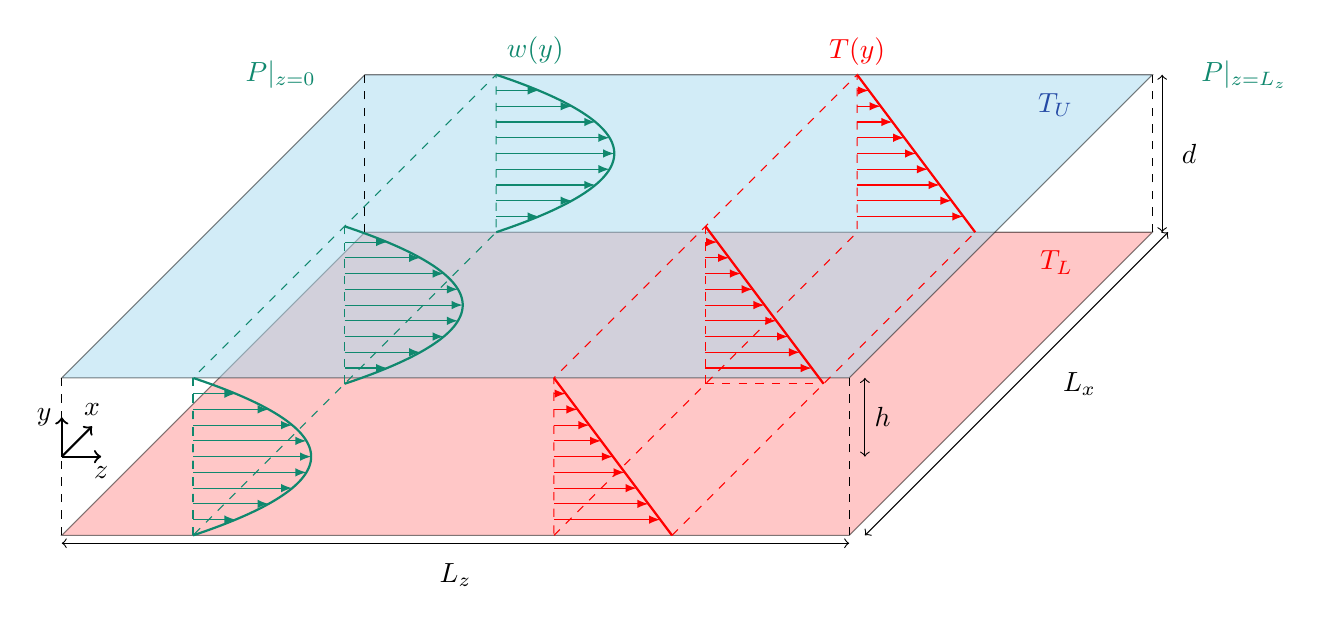
\begin{tikzpicture}
\def\H{1}
\def\W{10}
\def\L{10}

% Draw the bottom plate
\draw [fill=pink!75!red, opacity=0.5] (-\L/2,-\H,0) -- (\L/2,-\H,0) -- (\L/2, -\H, -\W) -- (-\L/2, -\H,-\W) -- cycle;

% Draw the top plate
\draw [fill=SkyBlue!75!white, opacity=0.5] (-\L/2,\H,0) -- (\L/2,\H,0) -- (\L/2, \H, -\W) -- (-\L/2,\H,-\W) -- cycle;

%  % Draw axes
\draw [dashed, thin] (-\L/2, -\H, 0) -- (-\L/2, \H, 0);
\draw [dashed, thin] (\L/2, -\H, 0) -- (\L/2, \H, 0);
\draw [dashed, thin] (\L/2, -\H, -\W) -- (\L/2, \H, -\W);
\draw [dashed, thin] (-\L/2, -\H, -\W) -- (-\L/2, \H, -\W);
%\draw [dashed, thin] (-1,0, 0) --++ (\L,0,0) --++ (0,0,-\W) --++ (-\L,0,0) -- cycle;
%  % \draw [thin, dashed] (-1,0) -- (6,0);

% Add dimensions
% L_x
\draw [<->] (-\L/2,-1.1*\H, 0) -- (\L/2,-1.1*\H,0);
\node[centered] at (0,-1.5*\H,0) {$L_z$};
 
% L_z
\draw [<->] (\L/2*1.025, -\H, -\W) -- (\L/2*1.025, \H,-\W);
\node[right] at (\L/2*1.05,0.0,-\W) {$d$};

% d
\draw [<->] (\L/2*1.04, -\H) -- (\L/2*1.04,-\H,-\W);
\node[centered] at (\L/2*1.2,-\H,-\W/2) {$L_x$};

% h
\draw [<->] (\L/2*1.04, 0, 0) -- (\L/2*1.04, \H, 0);
\node[right] at (\L/2*1.04,\H/2,0) {$h$};

% P
\node[left] at (-\L/2*1.1, \H, -\W) {\textcolor{PineGreen}{$P|_{z=0}$}};
\node[right] at (\L/2*1.1, \H, -\W) {\textcolor{PineGreen}{$P|_{z=L_z}$}};

% T
\node[left] at (\L/2*0.9, \H, -\W*0.9) {\textcolor{cyan!20!blue}{$T_U$}};
\node[left] at (\L/2*0.9, -\H, -\W*0.9) {\textcolor{red}{$T_L$}};

% Draw labels
\draw[->, thick] (-\L/2, 0, 0) -- (-\L/2,\H/2,0) node[left] {$y$};
\draw[->, thick] (-\L/2, 0, 0) -- (-\L/2+\H/2,0,0) node [below] {$z$};
\draw[->, thick] (-\L/2, 0, 0) -- (-\L/2,0,-\H) node[above] {$x$};

% Draw the velocity profile
\draw[PineGreen,thick,domain=-1:1,samples=200,smooth] plot ({(1-\x*\x)*1.5-\L/3}, \x) node[above right] {};
\draw[PineGreen,thick,domain=-1:1,samples=200,smooth] plot ({(1-\x*\x)*1.5-\L/3}, \x, -\W/2) node[above right] {};
\draw[PineGreen,thick,domain=-1:1,samples=200,smooth] plot ({(1-\x*\x)*1.5-\L/3}, \x, -\W) node[above right] {$w(y)$};
\draw[-,PineGreen,dashed] (-\L/3,-\H) -- (-\L/3,\H);
\draw[-,PineGreen,dashed] (-\L/3,-\H, -\W/2) -- (-\L/3,\H, -\W/2);
\draw[-,PineGreen,dashed] (-\L/3,-\H,0) -- (-\L/3,\H,0) -- (-\L/3,\H,-\W) -- (-\L/3,-\H,-\W) -- cycle;

\foreach \y in {-0.8,-0.6,...,0.8} {
    \draw[-latex,PineGreen] (-\L/3,\y, 0) -- ({(1-\y*\y)*1.5-\L/3},\y,0);
    \draw[-latex,PineGreen] (-\L/3,\y, -\W/2) -- ({(1-\y*\y)*1.5-\L/3},\y, -\W/2);
    \draw[-latex,PineGreen] (-\L/3,\y, -\W) -- ({(1-\y*\y)*1.5-\L/3},\y,-\W);
}

% Draw the temperature profile
\draw[red,thick,domain=-\H:\H,samples=200,smooth] plot ({(1/2*(1-\x)*1.5+\L/8)}, \x);
\draw[red,thick,domain=-\H:\H,samples=200,smooth] plot ({(1/2*(1-\x)*1.5+\L/8)}, \x, -\W/2);
\draw[red,thick,domain=-\H:\H,samples=200,smooth] plot ({(1/2*(1-\x)*1.5+\L/8)}, \x, -\W);
\draw[-,red,dashed] (\L/8,-\H,-\W/2) -- (\L/8,\H,-\W/2);
\draw[-,red,dashed] (\L/8,-\H,-\W/2) -- (\L/8 + 1.5,-\H,-\W/2);
\draw[-,red,dashed] (\L/8 +1.5,-\H,0) -- (\L/8 + 1.5,-\H,-\W);
\draw[-,red,dashed] (\L/8,-\H,0) -- (\L/8,-\H,-\W) -- (\L/8,\H, -\W) -- (\L/8,\H,0) -- cycle;
% % 
\foreach \y in {-0.8,-0.6,...,0.8} {
   \draw[-latex,red] (\L/8,\y) -- ({\L/8+(1/2*(1-\y)*1.5},\y);
   \draw[-latex,red] (\L/8,\y, -\W/2) -- ({\L/8+(1/2*(1-\y)*1.5},\y, -\W/2);
   \draw[-latex,red] (\L/8,\y, -\W) -- ({\L/8+(1/2*(1-\y)*1.5},\y, -\W);
}
% Add labels
\node[above,red] at (\L/8,1,-\W) {$T(y)$};
\end{tikzpicture}
\label{fig:rbpconfiguration}
\caption{The Rayleigh-B\'{e}nard Poiseuille (RBP) flow configuration.}
\end{figure}


The RBP configuration is illustrated in figure \ref{fig:rbpconfiguration}, where $z,x,y$ refer to spatial coordinates denoting the streamwise, spanwise and wall normal directions.
$L_z$, $L_x$, $d$, and $h$ correspond to the length, span, depth and half-height of the domain, respectively.
The RBP system is biperiodic along $z$ and $x$.
% We note that the asterisks$^*$, refer to variables in dimensional form.
The flow is driven by a pressure difference along the streamwise $z$ direction, $\Delta P = P|_{z=L_z} - P|_{z=0} < 0$, leading to a laminar Poiseuille flow, $w(y) = W_c(1 - y^2)$, where $W_c$ is the laminar centerline velocity.
We consider a fully developed flow, where the boundary layer developing from the top and the bottom wall meets at the midplane $y=0$ and entrance effects are therefore neglected.
Like the RBC system, the RBP system is unstably stratified.
The temperature difference between the lower, $T_L$, and upper wall, $T_U$, is always positive, $\Delta T = T_L - T_U > 0$, leading to a stable linear conduction layer along the wall-normal direction, $T(y)$, if $\Delta T$ is kept sufficiently small.
The behaviour of RBP flows is governed by four dimensionless parameters,
\begin{equation}\label{eq:nondim_def}
    Re = W_c h / \nu, \quad Ra = \frac{\eta g d^3 \Delta T}{\nu \kappa}, \quad Pr = \frac{\nu}{\kappa}, \quad \Gamma = L/2d,
\end{equation}
where $Ra, Re, Pr, \Gamma$ refer to the Reynolds, Rayleigh, Prandtl numbers and aspect ratio and $\eta, g, \nu, \kappa,$ are the thermal expansion coefficient, acceleration due to gravity, kinematic viscosity, and thermal diffusivity, respectively.
The Reynolds number, $Re$, and the Rayleigh number, $Ra$, are dimensionless parameters that characterise the relative influence of shear and buoyancy respectively.
For sufficiently large values of $Re$ and $Ra$, RBP flows may undergo a transition to shear-driven turbulence or buoyancy-driven convection.
In the absence of shear, $Re = 0$, the RBP configuration reduces to the classical buoyancy-driven Rayleigh-B\'{e}nard convection, which forms a bistable system between stationary and chaotic convection rolls slightly above the critical $Ra$.
The influence of $Re$ on bistability remains unexplored.

In the first part of this thesis, we focus on the transitional regime by investigating whether buoyancy forces promote the transition to shear-driven turbulence and examining the effect of shear on convection in large domains. 
The second part of this thesis explores the state space structure of a bistable system between a chaotic convection roll state and a stationary convection roll state (see spiral defect chaos and ideal straight rolls in \S \ref{sec:bkgrd_RBC}) of Rayleigh-B\'{e}nard convection.

The structure of this introductory chapter is as follows:
We begin our discussion on the development of hydrodynamic stability theory of wall-bounded shear flows in \S \ref{sec:bkgrd_transitional}.
Theoretical frameworks used in the study of the stability of fluid flow, including linear modal/non-modal stability, nonlinear dynamical systems and the spatio-temporal dynamics of transitional shear flows will be discussed.
Throughout \S \ref{sec:bkgrd_transitional}, we apply these concepts in the context of plane Poiseuille flows (PPF).
This is followed by the developments of Rayleigh-B\'{e}nard convection (RBC) in \S \ref{sec:bkgrd_RBC}.
Finally, we review the developments in RBP flows \S \ref{sec:bkgrd_RBP}, before concluding this chapter with the objectives of this thesis in \S \ref{sec:bkgrd_objs} and an outline of its structure in \S \ref{sec:bkgrd_outline}.


% We first discuss the key developments of plane Poiseuille flow (PPF) outlining the key theoretical framework for analysing the stability of fluid flows. This is then followed by Rayleigh-B\'{e}nard convection (RBC) in \S \ref{sec:bkgrd_RBC}.

%%%%%%%%%%%%%%%%%%%%%%%%
% Plane Poiseuille Flows
%%%%%%%%%%%%%%%%%%%%%%%%

\section{Transitional wall-bounded shear flows}\label{sec:bkgrd_transitional}
Wall-bounded shear flows concern the motion of the fluid flowing parallel to walls, typically bounded by one or more walls.
At the wall, the fluid comes to rest due to the no-slip boundary condition, resulting in a velocity gradient perpendicular to the wall, giving rise to shear within the fluid, commonly known as \textit{wall-bounded shear flows}.
Examples include the pressure-driven plane Poiseuille flow (channel flow), Hagen-Poiseuille flow (pipe flow), plane Couette flow and flat plate boundary layers.
These geometrically simple configurations provide a convenient framework amenable to the mathematical analysis of fluid motion under shear.
Depending on the degree of shear, the fluid motion can be either laminar, where the fluid layers move in smooth parallel laminates, or turbulent, characterised by chaotic eddying motions.
We also note a transitional regime in which both states can coexist.
A central question is the prediction of the transition from the laminar regime to turbulence.

The first investigation into this transition was conducted by \citet{reynolds_xxix_1883}.
% The earliest investigation into this transition dates back to the pipe flow experiments of \citet{reynolds_xxix_1883}.
In his experimental setup, Reynolds controlled the flow speed through the pipe by regulating the inlet pressure, and injected dye to visualise the flow, as illustrated in figure \ref{fig:reynolds}(a).
At low speeds, the fluid is laminar, resulting in a single streak of steady dye shown in figure \ref{fig:reynolds}(b).
As the speed is increased, the dye began to exhibit irregular `sinuous' motions interspersed with laminar regions shown in figure \ref{fig:reynolds}(c).
This is now referred to as the transitional regime, which alternates between laminar and turbulent states.
Beyond a critical speed, the dye breaks down entirely into chaotic eddies, mixing with the surrounding fluid and discolouring the flow with dye downstream, shown in figure \ref{fig:reynolds}(d).
This regime is now identified as turbulence.

Reynolds proposed that the threshold between the laminar, transitional and turbulent regimes could be characterised by a non-dimensional parameter, now referred to as the Reynolds number,
\begin{equation}
    Re = U D/\nu,
\end{equation}
where $U$ is the centerline velocity in the pipe, $D$, the pipe diameter and $\nu$, the kinematic viscosity.
He observed that flow through the pipe remained \textit{stable} and laminar for $Re < 1900$, while it became \textit{unstable} and turbulent for $Re > 2000$ \citep{reynolds_iv_1895}, introducing the notion of flow \textit{stability}.
\begin{figure}[h]
    \centering
    \includegraphics[width=1\textwidth]{Background/Figures/Reynolds.pdf}
    \caption{(a) Osbourne Reynolds pipe experiment with the dye injection apparatus, illustrating the (b) laminar flow, (c) transitional regime and (d) turbulent flow as the flow speed is increased, taken from \protect\citet{reynolds_xxix_1883}.}
    \label{fig:reynolds}
\end{figure}

%%%%%%%%%%%%%%%%%%%%%%%%%%%
% Linear Stability Analysis
%%%%%%%%%%%%%%%%%%%%%%%%%%%

\subsection{Linear Stability Analysis}
Following the experiment, interest towards the mathematical analysis of the stability of laminar flows grew in the early $20^{th}$ century.
The mathematical approach typically begins by decomposing the velocity field, $\mathbf{u}(\mathbf{x},t)$, into a laminar (base) state, $\mathbf{U}(\mathbf{x}) = U(y)\mathbf{e_x}$, and the velocity perturbations, $\mathbf{u}'(\mathbf{x},t)$, with pressure similarly decomposed as,
\begin{equation}
\mathbf{u}(\mathbf{x}) = \mathbf{U}(\mathbf{x}) + \mathbf{u}'(\mathbf{x},t), \quad \text{and} \quad p(\mathbf{x},t) = P(x) + p'(\mathbf{x},t).
\end{equation}
Substituting into the Navier-Stokes equations and linearising (neglecting nonlinear terms), we get,
\begin{subequations}\label{eq:shear_linearised}
\begin{equation}
    \frac{\partial \mathbf{u'}}{\partial t} + (\mathbf{U} \cdot\nabla)\mathbf{u'} + (\mathbf{u'}\cdot\nabla)\mathbf{U} = -\nabla p' + \frac{1}{Re}\nabla^2 \mathbf{u'},
\end{equation}
\begin{equation}
    \nabla \cdot \mathbf{u}' = 0,
\end{equation}
\end{subequations}
known as the linearised Navier-Stokes equations. 
This is commonly followed by introducing a wavelike ansatz (mode) for the perturbations, and analysed by considering their behaviour independently, referred to as modal analysis in \S \ref{subsec:modal}, or their coupled dynamics, referred to as non-modal analysis in \S \ref{subsec:nonmodal}.

%%%%%%%%%%%%%%%%%
% MODAL STABILITy
%%%%%%%%%%%%%%%%%

\subsubsection{Modal analysis}\label{subsec:modal}
It is convenient to eliminate the pressure term by reformulating equation \eqref{eq:shear_linearised} using the wall-normal perturbation velocity, $v'$, and wall-normal vorticity, $\eta' = \partial u'/ \partial z - \partial w' / \partial x$, variables.
Using $(v, \eta)$, we introduce a modal ansatz for them,
\begin{equation}\label{eq:shear_ansatz}
    v'(\mathbf{x},t ) = \tilde{v}(y)e^{i(\alpha x + \beta z - \omega t)} + \text{c.c}, \quad \text{and} \quad \eta'(\mathbf{x}, t) = \tilde{\eta}(y)e^{i(\alpha x + \beta z - \omega t)} + \text{c.c},
\end{equation}
where $\alpha, \beta, \omega$ and c.c denote the streamwise and spanwise wavenumbers, complex frequency (i.e. $\omega = \omega_r + i\omega_i$) and complex conjugate, respectively.
Substituting this ansatz into the linearised equations leads to the classical Orr-Sommerfeld and Squire equations \citep{orr_stability_1907,sommerfeld_beitrag_1909,squire_stability_1933, schmid_stability_2001},
% \begin{equation}
%     \mathbf{L}\mathbf{\tilde{q}} = i\omega\mathbf{M}\mathbf{\tilde{q}}
% \end{equation}
\begin{subequations}
\begin{equation}\label{eq:OSQ}
    \begin{pmatrix}
        \mathcal{L}_{OS} & 0 \\
        i\beta U' & \mathcal{L}_{SQ}
    \end{pmatrix}
    \begin{pmatrix}
        \tilde{v} \\
        \tilde{\eta}
    \end{pmatrix}
    = 
    i\omega
    \begin{pmatrix}
        k^2 - \mathcal{D}^2 & 0 \\
        0 & 1 
    \end{pmatrix}
    \begin{pmatrix}
        \tilde{v} \\
        \tilde{\eta}
    \end{pmatrix},
\end{equation}
\text{with}
  \begin{equation} 
      \mathcal{L}_{OS} = i\alpha U(k^2-\mathcal{D}^2) + i\alpha U'' + \frac{1}{Re}(k^2 - \mathcal{D}^2)^2,
      \quad \mathcal{L}_{SQ} = i\alpha U + \frac{1}{Re}(k^2 - \mathcal{D}^2),
  \end{equation}
\end{subequations}
where $\mathcal{D} = d/dy, k^2 = \alpha^2 + \beta^2$ and $U''$ is the second derivative of $U(y)$.
% $k^2, \mathcal{D}, U', U''$ denotes the sum of squared wavenumbers, $k^2 = \alpha^2 + \beta^2$, differential operator in $y$, first- and second- derivative of the laminar velocity, respectively.
Equation \eqref{eq:OSQ} is a generalised eigenvalue problem with eigenvalue $i\omega$, which determines the growth of perturbations.

The goal of modal stability analysis is to determine the critical Reynolds number $Re_c$, defined as the lowest value of $Re$, for all $\alpha$ and $\beta$ in which $\Im[\omega] = 0$.
For $Re > Re_c$, perturbations can grow exponentially, indicating instability.
% For $Re > Re_c$, perturbations could grow exponentially, departing from the laminar state.
% In other words, we consider the behaviour of each $\alpha-\beta$ mode independently, herein referred to as \emph{modal} analysis.
Squire's theorem states that for every unstable three-dimensional perturbation,  there exists an unstable two-dimensional perturbation, with a lower $Re_c$ \citep{squire_stability_1933}.
This implies that the most linearly unstable perturbation of wall-bounded flows is two-dimensional.
Calculations by \citet{tollmien_uber_1928} and \citet{schlichting_zur_1933} for a flat-plate boundary layer flow yielded a critical Reynolds number based on displacement thickness, $\delta^*$, of $Re_{ind} = U_\infty \delta^* / \nu = 520$ \footnote{In stability theory, $Re_{ind}$ refers to the indifference Reynolds number which is related to, but distinct from, the critical Reynolds number, $Re_{c}$ \citep{schlichting_onset_2017}. Because boundary layer transition occurs over a finite distance, the indifference point is introduced to distinguish between the onset of transition and the point at which the flow becomes fully turbulent.}
These two-dimensional unstable eigenmodes are known as Tollmien-Schlichting (T.S) waves.
In plane Poiseuille flow, the critical Reynolds number is $Re_{c} = 5772.2$ with a critical wavenumber of $\alpha_c = 1.02$ \citep{orszag_accurate_1971}.
However, experiments reveal that transition to turbulence can occur at a lower Reynolds number, around $Re \sim 1000 - 2000$ \citep{davies_experimental_1928, patel_observations_1969,dean_reynolds_1978,iida_relaminarization_1998,tsukahara_dns_2014}, highlighting a key limitation of modal analysis.
Similar discrepancies are observed in plane Couette and pipe flows \citep{meseguer_linearized_2003}, where the laminar state is linearly stable for all $Re$, yet transition to turbulence occurs.
Despite these limitations, modal analysis predicts instabilities in other systems such as Rayleigh-B\'{e}nard convection and Taylor-Couette flow \citep{chandrasekhar_stability_1968}.
Further extensions of modal stability, including spatial instability analysis \citep{huerre_local_1990}, and secondary instability \citep{orszag_secondary_1983} are well established and are beyond the scope of this thesis.

%%%%%%%%%%%%%%%%%%%%%
% Non-modal stability
%%%%%%%%%%%%%%%%%%%%%
\subsubsection{Non-modal stability}\label{subsec:nonmodal}
One of the major limitations of modal analysis is that it treats each eigenmode independently.
However, the interaction between decaying eigenmodes can lead to transient growth, in which perturbations amplify temporarily before decaying asymptotically.
\begin{figure}[h]
    \centering
    \includegraphics[width=\textwidth]{Background/Figures/PhasePotrait.pdf}
    \caption{(a) The phase portrait of the toy model with $Re = 15$, where red lines are phase lines of the toy model. The blue trajectory leads to transient growth and the green trajectory does not (b) Time history of blue and green trajectories.}
    \label{fig:toy_model}
\end{figure}
To demonstrate an example of transient growth, we consider a two-dimensional toy model governing the time-evolution of $\mathbf{q} = (v, \eta)^T$,
\begin{equation}
    \frac{\mathrm{d}}{\mathrm{d}t} \begin{pmatrix} v \\ \eta \end{pmatrix}  = \begin{pmatrix} -\frac{1}{Re} & -1 \\ 0 & -\frac{2}{Re} \end{pmatrix} \begin{pmatrix} v \\ \eta \end{pmatrix},
\end{equation}
where $Re$ refers to the Reynolds number.
The toy model has negative eigenvalues, $(\lambda_1, \lambda_2) = (-1/Re, -2/Re)$, indicating a linearly stable system where perturbations decay asymptotically.
At $Re = 15$, the eigenvectors, $\mathbf{x_1} = (1,0)$, $\mathbf{x}_2 = (1,\frac{1}{\sqrt{Re^2 + 1}})$, are highly non-orthogonal, becoming almost parallel, as shown in figure \ref{fig:toy_model}(a).
Notably, they become more linearly dependent as $Re \rightarrow \infty$.
For a particular initial condition, the energy, $||\mathbf{q}||_2 = \sqrt{v^2 + \eta^2}$, is amplified approximately four times before decaying, represented by the blue trajectory shown in figure \ref{fig:toy_model}(b).
Yet for another choice of initial condition, the trajectory decays asymptotically, as indicated by the green trajectory.
Despite the presence of decaying eigenmodes, the toy model highlights the importance of transient growth, which depends on the choice of initial conditions.

The aim of non-modal stability analysis is to search for optimal initial conditions, $\mathbf{\tilde{q}}_0$, that lead to the maximum amplification, $G(\tau)$, over a time horizon $\tau$. 
This is posed as an optimisation problem,
\begin{equation}\label{eq:transient_growth}
    % G(t) = \max_{\mathbf{\tilde{q}}_0 \neq 0 } \frac{||\mathbf{\tilde{q}}(t)||^2}{||\mathbf{\tilde{q}}_0||^2}, \quad \text{s.t} \quad ||\mathbf{\tilde{q}}_0||^2 = 1,
    G(\tau) = \max_{\mathbf{\tilde{q}}_0 \neq 0 } \frac{\langle \mathbf{\tilde{q}}(\tau), \mathbf{\tilde{q}}(\tau) \rangle }{\langle \mathbf{\tilde{q}}_0, \mathbf{\tilde{q}}_0 \rangle }, \quad \text{s.t} \quad \langle \mathbf{\tilde{q}}_0, \mathbf{\tilde{q}}_0 \rangle = 1,
\end{equation}
where, $\langle \cdot, \cdot \rangle$ denotes the inner-product,
\begin{equation}
    \langle \mathbf{\tilde{q}}, \mathbf{\tilde{q}} \rangle = \int_\Omega \mathbf{\tilde{q}}^H \mathbf{\tilde{q}} \; \mathrm{d}\Omega,
\end{equation}
and $\mathbf{\tilde{q}}^ H$ refers to the complex conjugate transpose of $\mathbf{\tilde{q}}$.
By considering the linearised operator of \eqref{eq:OSQ}, we define a linear operator as follows,
\begin{equation}\label{eq:linear_evolution}
    \mathbf{\tilde{q}}(\tau) = \mathcal{A}(\tau) \mathbf{\tilde{q}}_0,
\end{equation}
which takes the solution from initial conditions, $\mathbf{\tilde{q}}_0$, to $\mathbf{\tilde{q}}(\tau)$ at time $\tau$.
Substituting the expression above into equation \eqref{eq:transient_growth},
\begin{equation}\label{eq:transient_growth_adj}
    G(\tau) = \max_{\mathbf{\tilde{q}}_0 \neq 0 } \frac{\langle \mathcal{A}(\tau)\mathbf{\tilde{q}}_0, \mathcal{A}(\tau)\mathbf{\tilde{q}}_0 \rangle }{\langle \mathbf{\tilde{q}}_0, \mathbf{\tilde{q}}_0 \rangle} = \langle \mathbf{\tilde{q}}_0, \mathcal{A}^\dagger(\tau) \mathcal{A}(\tau)\mathbf{\tilde{q}}_0  \rangle \footnote{The adjoint, $\mathcal{A}^\dagger$, of operator, $\mathcal{A}$, statisfies the mathematical property of $\langle \mathcal{A} \mathbf{x}, \mathbf{y} \rangle = \langle \mathbf{x}, \mathcal{A}^\dagger\mathbf{y} \rangle$. By substituting $\mathcal{A}\mathbf{\tilde{q}_0}$ as $\mathcal{A}\mathbf{x}$, and $\mathcal{A}\mathbf{\tilde{q}_0}$ as $\mathbf{y}$, we arrive at $\langle \mathcal{A}(\tau)\mathbf{\tilde{q}_0}, \mathcal{A}(\tau)\mathbf{\tilde{q}_0} \rangle = \langle \mathbf{\tilde{q}_0}, \mathcal{A}(\tau)^\dagger \mathcal{A}(\tau)\mathbf{\tilde{q}_0}\rangle$.} = \lambda_{max} (\mathcal{A}^\dagger(\tau) \mathcal{A}(\tau)),
\end{equation}
where $\mathcal{A}^\dagger(\tau)$ is the adjoint of $\mathcal{A}(\tau)$.
The maximum amplification factor, $G(\tau)$, is the largest eigenvalue of $\mathcal{A}^\dagger(\tau)\mathcal{A}(\tau)$ and the corresponding eigenvector, $\mathbf{\tilde{q}}_0$, denotes the eigenvector.
The eigenvalue problem is given as,
\begin{equation}
    \mathcal{A}^\dagger(\tau)\mathcal{A}(\tau) \mathbf{\tilde{q}}_0 = \lambda \mathbf{\tilde{q}}_0.
\end{equation}
% where $\mathbf{\tilde{q}}_0$ refers to the eigenvector denoting the optimal initial condition.
For a detailed derivation of the optimal initial conditions or forcing, the reader is referred to \citet{butler_three-dimensional_1992} and \citet{schmid_nonmodal_2007}.
An alternative method for computing the optimal transient growth is to analyse the pseudospectra of the linear operators discussed in \citet{trefethen_pseudospectra_1997}.

Both two-and three-dimensional non-modal analyses reveal mechanisms for transient growth.
In two-dimensions, the optimal initial conditions are in the form of near-wall vortices tilted upstream, which amplifies transiently via the Orr-mechanism \citep{orr_stability_1907, farrell_optimal_1988,reddy_pseudospectra_1993}.
In three-dimensions, streamwise vortices are optimal, leading to the amplification of streamwise streaks via the well-known lift-up effect \citep{ellingsen_stability_1975,reddy_energy_1993}.
Notably, the spacing of these streaks analysed using non-modal analysis at higher Reynolds number has been consistently reported to occur around 100 wall units \citep{del_alamo_linear_2006,pujals_note_2009,hwang_linear_2010}, which supports experimental observations of streak spacing in turbulent boundary layers \citep{kline_structure_1967, smith_characteristics_1983}.

The main result of the non-modal analysis is that three-dimensional perturbations can lead to strong transient growth at subcritical Reynolds numbers, contradicting the two-dimensional TS waves predicted by modal analysis.
Both modal and non-modal mechanisms provide important insights into the linear mechanisms that may be responsible for the transition from laminar to turbulent flow.
\subsection{Nonlinear dynamical systems}\label{sec:bkgrd_nondysys}

In the previous section, we examined the laminar-to-turbulent transition using linear frameworks.
However, the transition process is ultimately described by the nonlinear Navier-Stokes equations, which motivates the development and adoption of mathematical frameworks beyond linear methods. 

In the context of shear flow turbulence, there has been a growing interest in adopting techniques from nonlinear dynamical systems, interpreting turbulence as a chaotic trajectory evolving within \textit{phase space}.
This \textit{phase space} is the set of all possible states of the flow that satisfy the Navier-Stokes equations, which \citet{hopf_mathematical_1948} formulated in an infinite-dimensional function space.
Later work showed that for finite viscosity, the long-term dynamics of the system often lie on a finite-dimensional \textit{manifold}, whose properties depend on the fluid viscosity.
A \textit{manifold} is a lower-dimensional subset of phase space that attracts long-term solution trajectories.
For large viscosity (i.e. low $Re$), this manifold reduces to a single point corresponding to the laminar state.
As viscosity is decreased (i.e. $Re$ is increased), this point may become linearly unstable, bifurcating to form new \textit{invariant solutions}. 
Examples of \textit{invariant solutions} (also called exact coherent states) are steady states (equilibria), travelling waves (or relative equilibria), periodic orbits and relative periodic orbits. 
An implication of this is that the transition to turbulence could be viewed as successive bifurcations from the laminar state, governed by a single control parameter (i.e. the Reynolds number), generalised by the so-called \textit{routes-to-chaos} scenarios.

\citet{landau_problem_1944} proposed that the transition to turbulence may occur through a sequence of Hopf bifurcations, each introducing a new incommensurate frequency, resulting in quasi-periodic motions on a high-dimensional torus.
However, this model did not capture the essential ingredients of turbulence, such as sensitivity to initial conditions and mixing \citep{john_routes_1993}.
\citet{ruelle_nature_1971} later shows that a \textit{strange attractor} exhibits the key features of chaos, can emerge after three successive Hopf bifurcations from a stationary state, referred to as the \textit{Ruelle-Takens} route to chaos.
This scenario has been observed in Taylor-Couette flow \citep{gollub_onset_1975}, and Rayleigh-B\'{e}nard convection \citep{swinney_transition_1978}.
Other routes-to-chaos scenarios, such as period-doubling \citep{feigenbaum_universal_1979} and intermittency \citep{manneville_intermittency_1979}, have been proposed.
For a review of these routes-to-chaos scenarios, the reader is referred to \citet{john_routes_1993}.
Nonetheless, the transition to turbulence is subcritical in shear flow configurations, meaning that the route-to-chaos scenarios do not always occur via bifurcations from the laminar state.

\begin{figure}[h]
    \centering
    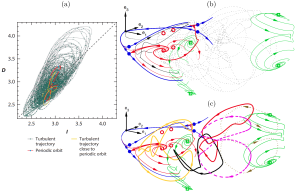
\includegraphics[width=\textwidth]{Background/Figures/BuildingBlocks.pdf}
    \caption{(a) Chaotic trajectory of turbulence of plane Couette flow at $Re = 400$ drawn in dark green. The yellow turbulent trajectory evolves close to an unstable periodic orbit in red,  adopted from \protect\citet{kawahara_periodic_2001}. (b) State space organisation of turbulence trajectories (black dots) confined around equilibria (circles, dots and squares) and their unstable manifolds (solid lines), heteroclinic connections between them are shown in red. The coordinate system, $(e_{1,2,3})$, is centered on the laminar state, using a linear combination of the upper branch invariant state. (c) State space projection of five periodic orbits (coloured solid lines), embedded within the same space where turbulence evolves in (b), adopted from \protect\citet{cvitanovic_geometry_2010}.}
    \label{fig:BuildingBlocks}
\end{figure}

A major development came with the identification of a pair of non-trivial, unstable equilibrium states in plane Couette flow \citep{nagata_three-dimensional_1990}.
This pair is referred to as the \textit{lower} and \textit{upper} branches, emerging from a saddle node bifurcation disconnected from the stable laminar state.
The \textit{lower} branch lies closer to the laminar state, while the \textit{upper} branch resides further away in state space.
% The lower branch refers to its proximity towards the stable laminar state in phase space.
Later, a travelling-wave solution in plane Couette flow was also found by the same author \citep{nagata_three-dimensional_1997}.
A family of equilibrium and travelling-wave solutions for plane Couette and plane Poiseuille flows with different boundary conditions (i.e., stress-free, slip, and no-slip) was later identified by \citet{waleffe_exact_2001} and \citet{waleffe_homotopy_2003}.
Additional equilibria and travelling-wave solutions were identified by \citet{gibson_visualizing_2008} and \citet{gibson_equilibrium_2009}, along with heteroclinic connections between them \citep{halcrow_heteroclinic_2009}.
In the context of pipe flow, multiple travelling-wave solutions have also been reported 
\citep{faisst_traveling_2003,wedin_exact_2004,kerswell_recurrence_2007,wang_lower_2007,duguet_transition_2008,pringle_highly_2009}.
The statistical quantities (e.g. mean and fluctuations) computed from the set of equilibria and travelling waves are in good agreement with those obtained from direct numerical simulations.
However, since these solutions are time independent (within a moving reference frame for travelling waves), they do not capture the temporal dynamics of turbulence such as the \textit{self-sustaining process} (SSP) \citep{hamilton_regeneration_1995} (see \S \ref{subsec:SSP}).


The next breakthrough was the identification of time-dependent unstable solutions in the form of periodic orbits. 
\citet{kawahara_periodic_2001} computed a pair of periodic orbits in plane Couette, with one exhibiting a single regeneration cycle similar to the SSP (see figure \ref{fig:BuildingBlocks}(a)) while the other exhibits mild modulation of streaks.
These periodic orbits are linked by heteroclinic connections.
In plane Poiseuille flow, \citet{toh_periodic-like_2003} also identified periodic orbits displaying bursting behaviour.
Using a Newton–Krylov iteration with a hook-step modification, \citet{viswanath_recurrent_2007} computed multiple relative periodic orbits.
These studies conceptualise that the chaotic trajectories of turbulence are embedded within a set of unstable periodic orbits, evolving along their unstable manifold \citep{viswanath_recurrent_2007,gibson_visualizing_2008,gibson_equilibrium_2009,halcrow_heteroclinic_2009,graham_exact_2021}.
An example is shown in figure \ref{fig:BuildingBlocks}, where the chaotic trajectories in figure \ref{fig:BuildingBlocks}(b), reside within the same state space as the periodic orbits, enclosed by equilibria and their heteroclinic connections shown in figure \ref{fig:BuildingBlocks}(c).
Chaotic trajectories of turbulence reside in the \textit{turbulent attractor} contains invariant solutions (e.g. equilibria, travelling waves, periodic orbits, and relative periodic orbits) that provide a building-block description of turbulence.
However, they invariant solutions do not provide insight into the transition process, since these solutions already reside in the turbulent attractor.

\begin{figure}[h]
    \centering
    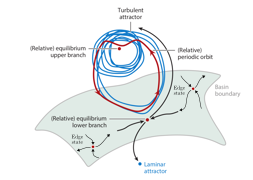
\includegraphics[width=0.8\textwidth]{Background/Figures/EdgeStates.pdf}
    \caption{A graphical representation of the \textit{basin boundary} (grey surface) that seperate the basins of attraction of the laminar and turbulent attractor. Along the basin boudary sit attractors, known as edge states, adapted from \protect\citet{graham_exact_2021}.}
    \label{fig:EdgeStates}
\end{figure}

The transition to turbulence in canonical shear flow configurations is typically subcritical, emerging from the invariant solutions described above, accompanied by an underlying stable laminar state.
A consequence of this is that the laminar and turbulent states form bistable attractors in phase space with a boundary, separating their respective basins of attraction, known as the \textit{basin boundary}.
Attractors that sit along this basin boundary were identified as saddles, attracting trajectories along the basin boundary and repelling them toward either towards the laminar or turbulent state, known as \textit{edge states}.
The bisection algorithm for edge tracking was first applied to pipe-flow experiments by \citet{schneider_turbulence_2007}.
The edge state was found to be chaotic. 
It was shown that the time-averaged edge state is similar to the unstable lower-branch travelling-wave solutions, suggesting that the basin boundary contains lower branch solutions and their symmetries in pipe flows \citep{duguet_transition_2008,pringle_highly_2009}.
As the Reynolds number increases, the separation between the edge state and the turbulent attractor moves apart \citep{schneider_edge_2009}.
A graphical representation of the basin boundary and edge states separating the basin of attractions of the laminar and turbulent states is shown in figure \ref{fig:EdgeStates}.

Near the onset of subcritical turbulence, turbulence appears to be transient, decaying towards the laminar solution after a finite lifetime \citep{bottin_discontinuous_1998,faisst_sensitive_2004,hof_finite_2006}.
From a dynamical-system perspective, this can be interpreted as the turbulent chaotic attractor colliding with the lower branch solution known as a \textit{boundary crisis} \citep{lai_transient_2011}, forming a \textit{chaotic saddle} where solution trajectories may leak (relaminarise) towards the laminar state \citep{mellibovsky_travelling_2012, kreilos_periodic_2012, zammert_crisis_2015}.
The onset of a boundary crisis (transient turbulence) has also been attributed to the emergence of homoclinic tangency in plane Couette flow \citep{van_veen_homoclinic_2011,lustro_onset_2019}.

%%%%%%%%%%%%%%%%%%%%%%%%%%%%%%%%%%%
% The self-sustaining process 
%%%%%%%%%%%%%%%%%%%%%%%%%%%%%%%%%%%
\subsection{Self-sustaining process}\label{subsec:SSP}
\begin{figure}[h]
    \centering
    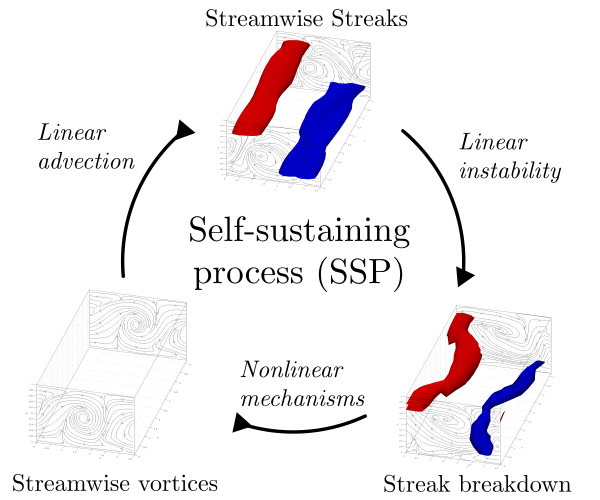
\includegraphics[width=0.7\textwidth]{Background/Figures/SSP/SSP.pdf}
    \caption{The self-sustaining process, consisting of three phases: (1) Streak formation from linear advection by streamwise vortices, (2) streak breakdown due to streak instability and (3) regeneration of streamwise vortices via nonlinear mechanisms.}
    \label{fig:SSP}
\end{figure}

The self-sustaining process (SSP) describes the dynamical interaction between a pair of streaks and quasi-streamwise vortices, which is considered the fundamental process in wall-bounded turbulent flows in the near-wall region.
It is defined by a quasi-cyclic process, consisting of three distinct phases: (1) the formation of streamwise streaks due to a linear advection by streamwise vortices, (2) the wavy breakdown of streaks due to linear instability and (3) the regeneration of streamwise vortices via nonlinear mechanisms \citep{durst_origin_1993,hamilton_regeneration_1995,waleffe_self-sustaining_1997}.
A schematic of the SSP is shown in figure \ref{fig:SSP}.
While early investigations of the SSP were confined to the buffer layer \citep{hamilton_regeneration_1995}, evidence that the SSP extends towards the logarithmic and outer region has been found \citep{cossu_self-sustaining_2017}.
In parallel to the SSP, the vortex-wave interaction (VWI) theory developed to describe the sustained interactions between a general class of vortices and waves for asymptotically large Reynolds number \citep{hall_nonlinear_1988,stewart_near-planar_1990,hall_strongly_1991}, was found to be linked to the SSP \citep{hall_streamwise_2010}.
In particular, the solutions obtained using VWI theory by \citet{hall_streamwise_2010} are analogous to the lower branch solutions from \citet{wang_lower_2007}.

%%%%%%%%%%%%%%%%%%%%%%%%%%%%%%%%%%%
% Spatiotemporal transitional flows
%%%%%%%%%%%%%%%%%%%%%%%%%%%%%%%%%%%

\subsection{Spatiotemporal transitional flows}
\begin{figure}[h]
    \centering
    \includegraphics[width=1.05\textwidth]{Background/Figures/Re1400.pdf}
    \caption{A snapshot of turbulent-laminar bands at $Re = 1400$ in a large domain $L/h = 16\pi$, depecting its spatiotemporal intermittent nature. Isovolume renderings are based on the spanwise, $u'$, and wall-normal, $v'$, perturbation kinetic energy, $E(u',v') = 1/2(u'^2 + v'^2)$, where the perturbation velocities are defined about the laminar state $\mathbf{u}'(\mathbf{x},t) = \mathbf{u}(\mathbf{x},t) - U_{lam}(y)$.}
    \label{fig:turbulent-laminar}
\end{figure}

This section describes the inherent spatiotemporal structure of subcritical turbulence near the onset commonly reported in large extended domains.
In this regime, turbulence is characterised by the coexistence of turbulent and laminar flow structures.
Examples of such are found in canonical shear flow systems such as plane Couette flows \citep{prigent_long-wavelength_2003,barkley_computational_2005,barkley_mean_2007,tuckerman_patterns_2011,duguet_formation_2010,reetz_exact_2019}, Taylor-Couette flows \citep{prigent_barber_2002,prigent_long-wavelength_2003}, pipe flows \citep{avila_transient_2010,avila_onset_2011,song_speed_2017,avila_transition_2023} and plane Poiseuille flows \citep{tsukahara_dns_2014, tsukahara_dns_2014-1, tuckerman_turbulent-laminar_2014, tsukahara_experimental_2014, gome_statistical_2020, paranjape_onset_2019, paranjape_oblique_2020, paranjape_direct_2023}.

We will focus on the plane Poiseuille flow configuration, where the spatiotemporal intermittent patterns are referred to as oblique turbulent-laminar bands illustrated in figure \ref{fig:turbulent-laminar} at $Re = 1400$ for $L/h = 16\pi$.
The bright and dark regions highlight coexisting spatially-localised turbulent and laminar regions.
These turbulent-laminar bands occur over a range of Reynolds numbers, and their precise range is dependent on the domain's aspect ratio \citep{tsukahara_experimental_2014,tuckerman_turbulent-laminar_2014,paranjape_direct_2023}.
Near the upper $Re$ threshold of this regime, the domain is fully engulfed by uniform, featureless turbulence appearing at $Re = 1800$ in figure \ref{fig:turbulent-laminar}.
As $Re$ decreases towards $Re = 1050$, spatiotemporal turbulent and laminar structures known as turbulent-laminar bands persist in between $Re \in [1050, 1600]$ shown in figures \ref{fig:turb_lam_bands}(b-f).
In particular, these turbulent-laminar bands appear to have a preferred inclined angle, between $20^\circ \sim 30^\circ$, with streamwise wavelengths of $\lambda_x \sim 60h$, and spanwise wavelengths of $\lambda_z \sim 20h-30h$ \citep{tsukahara_experimental_2014}.
\citet{kashyap_linear_2022} considered the linear response of the fluctuating turbulent field, and showed that the preferred band angle emerges near $23.2^\circ$.
In the minimal band unit (MBU) studies of plane Poiseuille flows, the turbulent-laminar bands convect at about $\sim1\%$ of the bulk velocity, propagating either upstream or downstream, depending on $Re$ \citep{tuckerman_turbulent-laminar_2014,gome_statistical_2020}.
Notably, the spanwise lengths of the bands are much wider than the half-heights and depend on $Re$, appearing at $\lambda_z \sim 20h$ for $Re \gtrsim 1400$ and $\lambda_z \sim 40h$ for $Re \lesssim 1100$.
Interestingly, the bands alternate between both spanwise lengths within $1100 \lesssim Re \lesssim 1400$ , merging and splitting continuously \citep{tuckerman_turbulent-laminar_2014}, reminiscent of a puff splitting process in pipe flows \citep{avila_onset_2011}.
An example of this could been observed in $Re = 1050$, where the band appears to alternate between different spanwise wavelengths in figure \ref{fig:turb_lam_bands}(f).
% Below certain $Re$ threshold, the spatially turbulent regions decay where the flow relaminarises \citep{tuckerman_turbulent-laminar_2014}.
As $Re$ falls below a certain $Re$ threshold, turbulent bands spontaneously decay and relaminarise \citep{tuckerman_turbulent-laminar_2014,gome_statistical_2020}.
An example is shown in figure \ref{fig:turb_lam_bands}(g).
% An example of this decay is shown in $Re = 1000$ near $t = 1600$ in figure \ref{fig:turb_lam_bands}(g). 
\begin{figure}[h]
    \centering
    \includegraphics[width=\textwidth]{Background/Figures/Ra0-BotSpaceTime.pdf}
    \caption{Turbulent-laminar bands for $t \in [0, 3000]$ in large domains $(L_x, L_z) = (16\pi, 16\pi)$ at (a) $Re = 1800$, (b) $Re = 1600$, (c) $Re = 1400$,  (d)  $Re =1200$, (e) $Re = 1100$, (f) $Re = 1050$,  (g) $Re = 1000$.}
    \label{fig:turb_lam_bands}
\end{figure}

\begin{figure}[h]
    \centering
    \includegraphics[width=0.7\textwidth]{Background/Figures/gome_prob.pdf}
    \caption{The mean decay times (red), $\tau^d$, and mean splitting times (black), $\tau^s$, as a function of Reynolds number, leading to a crossover point at $Re_{cross} \approx 965$, adapted from \protect\citet{gome_statistical_2020}.}
    \label{fig:decay_split_probability}
\end{figure}

\citet{gome_statistical_2020} computed the probability distributions for turbulent-laminar band decay, $P(\Delta t^d)$, where $\Delta t^d$ is the time until decay.
A key insight is that the probability distribution of turbulent band decay is a memoryless Poisson process,
\begin{equation}
    P(\Delta t^d) = \exp(-\Delta t^d/\tau^d(Re)),
\end{equation}
where $\tau^d(Re)$ refers to the mean lifetime for decay as a function of $Re$.
Similarly, the band splitting process also follows a Poisson process,
\begin{equation}
    P(\Delta t^s) = \exp(-\Delta t^s / \tau^s(Re)),
\end{equation}
while $\tau^s(Re)$ is the mean splitting lifetime.
Both $\tau^d$ and $\tau^s$ exhibit superexponential dependence on $Re$, shown in figure \ref{fig:decay_split_probability} (see inset).
The crossover point, $Re_{cross} \approx 965$, where both band decay and splitting events become equally probable, is considered the critical Reynolds number for the onset of turbulent-laminar bands.

While there has been progress made towards our understanding of infinitely bi-periodic turbulent-laminar bands in MBUs, recent studies of isolated (non-periodic) turbulent bands (ITBs) reveal different behaviour.
Notably, ITBs persist at Reynolds number below $Re_{cross}$ at $Re = 700$ for durations exceeding $t = 10000$, exceeding the mean decay lifetime in figure \ref{fig:decay_split_probability}.
The ITBs are characterised by a streak-generating head and a diffuse upstream tail. \citep{xiong_turbulent_2015, tao_extended_2018, shimizu_bifurcations_2019, xiao_growth_2020}.


%%%%%%%%%%%%%%%%%%%%%%%%%%%%
% Rayleigh Benard Convection
%%%%%%%%%%%%%%%%%%%%%%%%%%%%

\section{Rayleigh-B\'{e}nard convection}\label{sec:bkgrd_RBC}

\begin{figure}[h]
    \centering
    \includegraphics[width=\textwidth]{Background/Figures/BenardCells.png}
    \caption{(a) Surface tension driven convection leading to the onset of hexagonal B\'{e}nard cells in a thin layer of silicone oil, heated from below and cooled by ambient air. A diamond defect appears, likely caused by plate imperfections. (b) Buoyancy driven convection between rigid plates, resulting in concentric convection rolls at $2.9$ times the critical Rayleigh number. Both experiments were performed by \protect\citet{koschmieder_heat_1974}, and the convection patterns were illuminated by aluminum powder, where the dark and bright regions refer to vertical and horizontal motions respectively. These higher resolution images were taken from \protect\citet{van1982album}.}
    \label{fig:benard_cells}
\end{figure}

Rayleigh-B\'{e}nard convection (RBC) is a paradigmatic fluid configuration describing the motion of the fluid confined between two infinite-parallel plates heated from below and cooled from the top.
% The basic physical mechanism underpinning RBC is variation of buoyancy due to heat, offering a simple description of natural convection.
As the bottom plate is heated, the bottom-layer fluid becomes more buoyant and tends to rise, whereas the colder top-layer fluid becomes less buoyant and tends to sink, leading to overturning of the layers.
Viscous forces between neighbouring fluid parcels act to resist the motion. 
As buoyancy overcomes these viscous forces, the fluid layers overturn, initiating buoyancy-driven convection, the physical mechanism underpinning RBC.

One of the earliest experimental studies dedicated to buoyancy-driven convection was conducted by Henri B\'{e}nard \citep{benard_tourbillons_1901}, who observed the formation of hexagonal convection cells above a certain temperature threshold $\Delta T$.
These hexagonal patterns are referred to as B\'{e}nard cells, illustrated in figure \ref{fig:benard_cells}(a). 
Subsequently, \citet{rayleigh_lix_1916} carried out one of the first linear stability analyses of buoyancy-driven convection, predicting the onset of convection at a critical Rayleigh number of $Ra_c = 657.5$.
However, Rayleigh's analysis assumed idealised free-free boundary conditions, which differed from the rigid-free setup of B\'{e}nard's experiment.
The linear stability analysis for the rigid-free configuration was later performed by \citet{jeffreys_cases_1928}, yielding a higher critical Rayleigh number of $Ra_c = 1058$.
In the rigid-rigid configuration, the critical Rayleigh number increases further to $Ra_c = 1708$ \citep{pellew_maintained_1940}.
The Rayleigh number in B\'{e}nard's original experiment contradicted results from linear stability analysis as it was found to be 300 to 1500, smaller than $Ra_c$ for the free-free and rigid-free cases respectively \citep{wesfreid_henri_2017}.
This contradiction, not recognised by B\'{e}nard at the time, lies in the significant role of surface tension in thin fluid layers exposed to air, now known as B\'{e}nard-Maragoni (BM) convection \citep{block_surface_1956, cloot_nonlinear_1984, hohler_rayleigh-benard_2006, wesfreid_henri_2017}.
In BM convection, fluid motion is primarily driven by surface tension gradients due to variations of temperature, forming hexagonal cells, as in figure \ref{fig:benard_cells}(a).
The preference for hexagonal cells in BM convection was later confirmed based on weakly nonlinear stability analysis \citep{cloot_nonlinear_1984}.
As the fluid layer becomes thicker, surface-tension effects diminish and buoyancy-driven convection becomes dominant.
Similarly, placing a rigid lid on top of a thin fluid layer suppresses surface-tension effects, resulting in buoyancy-driven convection (compare between \ref{fig:benard_cells}(a) and (b))
The preferred convection patterns based on weakly nonlinear stability analysis are the two-dimensional parallel rolls, now referred to as ideal straight rolls (ISRs) \citep{schluter_stability_1965, bodenschatz_recent_2000}.
In circular containers, the ISRs conform to the geometry of the boundaries, forming concentric convection rolls illustrated in figure \ref{fig:benard_cells}(b).
Interestingly, hexagonal cells have been observed in buoyancy-driven flows of non-Boussinesq fluids \citep{hoard_experiments_1970,bodenschatz_recent_2000}.
In this thesis, we consider the RBP setup (and RBC in chapter 4) with rigid-rigid boundary conditions and a critical Rayleigh number of $Ra_c = 1708$.
Notably, the corresponding critical wavelength is $q_c = 3.12 / d$ (or $\lambda_c \approx  2d$), suggesting that the distance separating the plates, $d$, dictates the length of a single roll, $l_{roll} = \lambda_c / 2 \approx d$.

\begin{figure}[t]
    \centering
    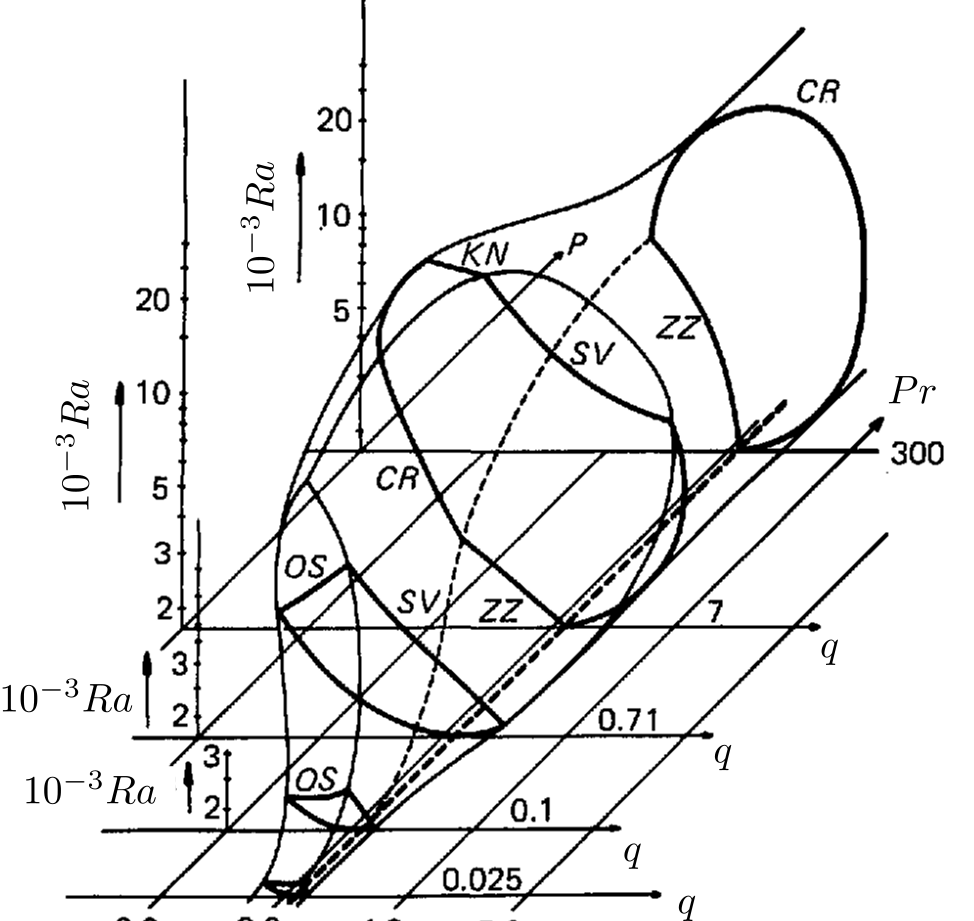
\includegraphics[width=0.8\textwidth]{Background/Figures/BusseBalloon_Busse.png}
    \caption{The Busse balloon describes the stability boundaries of ISRs in a $Ra-Pr-q$ space. For large values of $Pr$, the instability mechanisms are the cross-roll (CR), knotted (KN) and zig-zag (ZZ) instabilities. For $Pr\approx1$, the instability mechanisms are the skew-varicose (SV) and oscillatory (OS) instability. For small values of $Pr$, the OS instability dominants. This figure was modified from \protect\citet{swinney_transition_1981}.}
    \label{fig:busseballon}
\end{figure}

As mentioned earlier, stationary ISRs near $q_c$ emerge just above $Ra_c$, based on weakly nonlinear stability analysis \citep{eckhaus_studies_1965, schluter_stability_1965}.
However, this prediction is contradicted by the emergence of time-dependent oscillatory convection rolls in experiments \citep{rossby_study_1969,willis_oscillatory_1970} at $Ra = 9200$ (or roughly five times $Ra_c$), where weakly nonlinear stability analysis becomes inapplicable far from threshold.
To address this, secondary stability analysis was performed to study the stability of ISRs further from $Ra_c$ \citep{busse_oscillatory_1972}.
One of the key results from this analysis is the Busse balloon, which describes the stability boundaries of ISRs as a function of $Ra$ and $Pr$, and roll wavenumber, $q$, shown in figure \ref{fig:busseballon} \citep{swinney_transition_1981}.
The boundaries of the Busse balloon are described by a range of secondary instabilities, each arising from different physical mechanisms \citep{busse_non-linear_1978}.
At large Prandtl numbers, $Pr = O(10^2)$, the zig-zag (ZZ) and cross-roll (CR) instabilities delimit the balloon for small and large roll wavenumbers.
The zig-zag instabilities cause zig-zag undulations while the CR instabilities generate rolls orthogonal to the underlying ISR structure, effectively increasing or decreasing the roll wavenumber, respectively \citep{busse_instabilities_1971}.
Examples of these instabilities at $Pr = 100$ are illustrated in figure \ref{fig:busseballoon_secinstab}(a,b).

\begin{figure}
    \centering
    \includegraphics[width=0.5\textwidth]{Background/Figures/BusseBalloon/SecondaryInstabilities.pdf}
    \caption{ISRs experiencing (a) cross-roll instability at $Ra = 3000, Pr = 100$ and (b) zig-zag instability at $Ra = 3600, Pr = 100$ \protect\citep{busse_instabilities_1971}. (c) Skewed-varicose instability at $Ra = 5568, Pr = 1$ \protect\citep{plapp_spiral_1997}, and (d) oscillatory instability at $Ra = 10384, Pr = 1$ \citep{cakmur_bistability_1997}.}
    \label{fig:busseballoon_secinstab}
\end{figure}

At moderate Prandtl numbers, $Pr = O(1)$, the Busse balloon is bounded by the skew-varicose (SV) for high roll wavenumbers and the oscillatory (OS) instability at large $Ra$.
The skew-varicose (SV) instability leads to roll-pinching, where pinched rolls merged into a single roll, reducing roll wavenumber, while the oscillatory instability leads to the onset of an oscillatory convection roll. 
Examples of the respective instabilities at $Pr = 1$ are shown in figure \ref{fig:busseballoon_secinstab}(c,d).
At higher wavenumbers, the skew-varicose (SV) instability becomes relevant at intermediate Prandtl numbers, characterised by roll pinching and merging that effectively reduces the roll wavenumber.
% For larger Rayleigh numbers and $Pr \lesssim 1$, the oscillatory instability (OS) arises, forming oscillatory ISRs \citep{willis_oscillatory_1970}.
% In contrast, for higher $Pr$, the knot instability appears, modifying the cross-roll pattern into a spoke-like structure.
Finally, the Eckhaus instability (not shown), which either creates or destroys rolls such that the resultant roll wavenumber moves closer to the critical wavenumber, appears close to $Ra_c$ \citep{lowe_pattern_1985}.
Near $Pr = 1$, the Eckhaus instability coincides with the cross-roll instability (figure 6 from \citet{bodenschatz_recent_2000}, adapted from \citet{plapp_spiral_1997}).

In this thesis, we focus on fluids with $Pr = 1$, where secondary instabilities such as skew-varicose, Eckhaus and cross-roll instabilities typically arise.
While the stability boundaries of the Busse balloon have been experimentally verified \citep{busse_instabilities_1971, croquette_convective_1989, plapp_spiral_1997}, accurately predicting the wavenumber of ideal straight rolls (ISRs) remains difficult due to hysteresis and the existence of multiple stable ISRs of different roll wavenumbers.
As $Ra$ is increased, ISRs with wavenumbers outside the Busse Balloon undergo secondary instabilities (described above) that drive their wavenumbers back towards the stable boundaries.
The hysteretic behaviour highlights that the roll wavenumber of ISRs is strongly dependent on the system's history \citep{bodenschatz_recent_2000}.

% MULTIPLE STATES
It is worth noting that the ISRs are the exception rather than the rule in RBC \citep{croquette_convective_1989-1}.
A range of non-ISR states, such as squares, travelling or stationary target patterns, giant rotating spirals, and oscillatory convection, have been observed over the years \citep{le_gal_square_1985, croquette_convective_1989, plapp_spiral_1997, hof_flow_1999, rudiger_pattern_2000, boronska_extreme_2010_A, boronska_extreme_2010_B}.
For example, \citet{hof_flow_1999} identified eight stationary and two oscillatory states in cylindrical RBC with small aspect ratios at the same Rayleigh number.
These results were later verified in numerical simulations and bifurcation analysis, revealing up to twelve stable branches near the onset ($Ra \leq 2500$) and the potential for hundreds more as $Ra$ is increased \citep{ma_multiplicity_2006,boronska_extreme_2010_A,boronska_extreme_2010_B}.

In larger domains ($\Gamma \geq 28$), giant rotating spirals were found and have been investigated \citep{plapp_core_1996, plapp_dynamics_1998}.
Experimental and numerical studies of RBC with varying sidewall boundary conditions (i.e. thermally insulating, conducting and no-slip) \citep{tuckerman_global_1988, siggers_dynamics_2003, paul_pattern_2003,boulle_bifurcation_2022}, non-Boussinesq convection \citep{bodenschatz_experiments_1992}, and rotational effects \citep{hu_convection_1997} were investigated, where multiple states were also reported.
In inclined RBC, \citet{reetz_invariant_2020} and \citet{reetz_invariant_2020-1} identified up to sixteen stable and unstable invariant states, along with heteroclinic orbits connecting them.
These findings indicate that RBC supports a wide variety of coexisting stable states beyond ISRs, resulting in a system with multiple stable states above the critical Rayleigh number.
To further complicate matters, RBC also exhibits spatiotemporal chaos.
\begin{figure}[h]
    \centering
    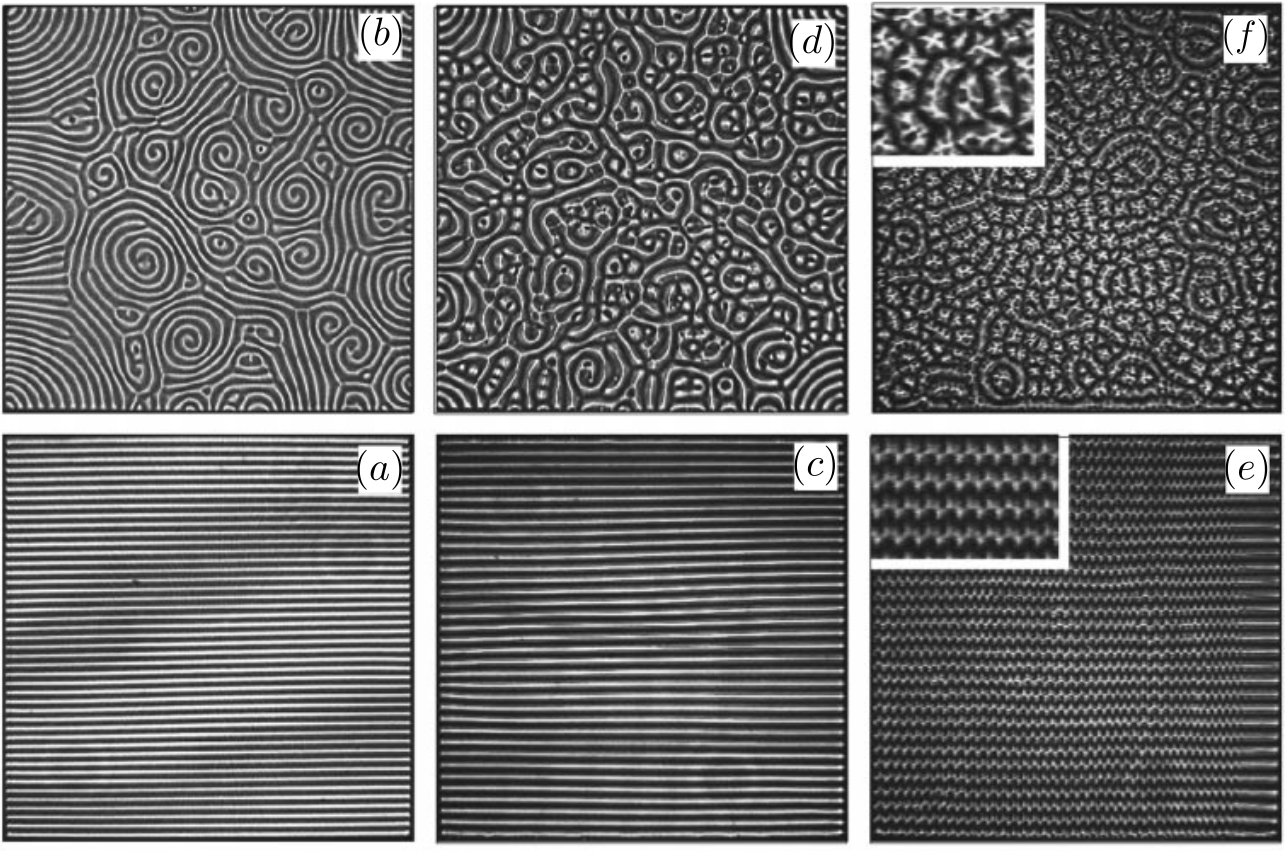
\includegraphics[width=0.8\textwidth]{Background/Figures/bistability.png}
    \caption{The coexistence of spiral defect chaos (SDC, top row) and ideal straight rolls (ISRs, bottom row) at (a,b) $Ra = 3279$, (c,d) $Ra = 6832$ and (e,f) $Ra = 10384$. The domain size is $\Gamma = 50$ and $Pr = 1$, adapted from \protect\citet{cakmur_bistability_1997}.}
    \label{fig:sdc_isr}
\end{figure}

% SDC
In the 1990s, convection rolls exhibiting spatio-temporal chaotic behaviour known as spiral defect chaos (SDC) were observed within the same stability boundaries where ISRs were expected \citep{morris_spiral_1993, hu_convection_1993,decker_spiral_1994,hu_convection_1995,morris_spatio-temporal_1996,cakmur_bistability_1997,ahlers_experiments_nodate,egolf_importance_1998,egolf_mechanisms_2000,chiam_mean_2003,vitral_spiral_2020}.
Notably, ISRs emerge with carefully prepared initial conditions, while uncontrolled initial conditions lead to SDC.
It is now well established that SDC exists as an intrinsic attractor of RBC, independent of sidewall conditions \citet{morris_spatio-temporal_1996}, forming a bistable system with ISRs \citep{cakmur_bistability_1997} across a range of $Ra$ at $Pr = 1$ illustrated in figure \ref{fig:sdc_isr}.
At $Pr = 4$, SDC appears to be transient, decaying towards ISRs over long periods, suggesting that the bistable system is $Pr$ dependent \citep{bajaj_competition_1997}.
SDC has also been replicated in numerical simulations using two-dimensional Swift-Hohenberg equations \citep{swift_hydrodynamic_1977,xi_spiral_1993,xi_spatiotemporal_1995,schmitz_spiral-defect_2002,karimi_exploring_2011}.
The critical Rayleigh number for the onset of SDC, $Ra_s$, depends on the domain's aspect ratio, and Prandtl number \citep{hu_convection_1995,bajaj_competition_1997,cakmur_transition_1997,bodenschatz_recent_2000}.
% Investigations into quantifying the onset of SDC in terms of Rayleigh number remain inconclusive as it appears to depend on the domain's aspect ratio, and Prandtl number \citep{hu_convection_1995,bajaj_competition_1997,cakmur_transition_1997,bodenschatz_recent_2000}.
% The critical reduced Rayleigh number for the onset of SDC, $\varepsilon_s$, has been observed to decrease with increasing $\Gamma$, and increase with increasing $Pr$ \citet{hu1995a, hu1995b, bajaj1997, Cakmur97, bodenschatz2000}.
SDC has been primarily reported in large aspect ratio domains ($\Gamma \gtrsim 20$), suggesting that a minimal domain size is required for SDC to occur \citep{bodenschatz_recent_2000}.
This is consistent with the leading Lyapunov exponents of SDC, which increases with $\Gamma$ \citep{egolf_mechanisms_2000, paul_extensive_2007}.
To characterise SDC, several studies have investigated its spatial-temporal properties, such as the averaged roll-curvature \citet{hu_convection_1995}, probability distribution of spirals \citep{ecke_excitation_1995, liu_spiral-defect_1996} and correlation length-/time-scales \citep{morris_spiral_1993, morris_spatio-temporal_1996, cakmur_transition_1997}.
Specifically, the correlation length-scales were found to grow exponentially \citep{morris_spiral_1993, morris_spatio-temporal_1996, cakmur_transition_1997}, suggesting that the transition from ISRs to SDC is related to phase transitions.
Similar SDC-like patterns have been observed in rotating RBC \citep{hu_convection_1997}, dielectric barrier discharge \citep{dong_observation_2005} and advection diffusion reaction systems \citep{affan_spiral_2014}.

%%%%%%%%%%%%%%%%%%%%%%%%%%%%%%%%%%
% Rayleigh Benard Poiseuille flows
%%%%%%%%%%%%%%%%%%%%%%%%%%%%%%%%%%

\section{Rayleigh-B\'{e}nard Poiseuille (RBP) flows}\label{sec:bkgrd_RBP}

\begin{figure}[h]
    \centering
    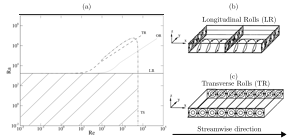
\includegraphics[width=\textwidth]{Background/Figures/RBP/RBP.pdf}
    \caption{(a) Neutral stability curves of longitudinal rolls (LR), oblique rolls (OR), transverse rolls (TR) and Tollmien-Schlicting (TS) waves, adapted from \protect\citet{john_soundar_jerome_transient_2012}. The shaded area refers to a linearly stable region. Sketch of (b) longitudinal and (c) transverse rolls, adapted from \protect\citet{kelly_onset_1994}.}
    \label{fig:primary_instabilities}
\end{figure}
This section describes the developments of Rayleigh-B\'{e}nard Poiseuille (RBP) flows, integrating key findings from both plane Poiseuille flow (PPF) and Rayleigh-B\'{e}nard convection (RBC) systems discussed in \S \ref{sec:bkgrd_transitional} and \S \ref{sec:bkgrd_RBC} respectively.
The neutral stability curves in the Rayleigh-B\'{e}nard Poiseuille (RBP), comprising both plane Poiseuille flow (PPF) and Rayleigh-B\'{e}nard convection (RBC) systems, are bounded by the onset of Tollmien-Schlicting waves at $Re_{c} = 5772.22$ \citep{orszag_accurate_1971}, and by the onset of convection rolls at $Ra_c = 1708$ \citep{pellew_maintained_1940}, respectively.
In RBP systems, the imposed mean Poiseuille flow in the RBP system breaks the rotational symmetry of the convection rolls, categorising them based on their orientation to the mean flow direction, namely: longitudinal, transverse and oblique rolls.
These primary instabilities were first investigated by \citet{gage_stability_1968} in an infinitely extended layer.
For longitudinal rolls, the linearised system reduces to the classical RBC problem.
Thus, the critical Rayleigh number remains unchanged at $Ra_{\parallel} = Ra_{c} = 1708.8$ with a critical wavenumber, $\alpha_{\parallel} = \alpha_{c} = 3.13$, independent of Reynolds number and Prandtl number \citep{pellew_maintained_1940, kelly_onset_1994}.
In contrast, the critical Rayleigh number for the onset of transverse rolls increases with $Re$, and is also dependent on $Pr$ \citep{gage_stability_1968, muller_transversal_1992, nicolas_two-dimensional_1997}.
The critical Rayleigh number for the onset of oblique rolls can be obtained by applying Squire's transformation \citep{squire_stability_1933} to the transverse roll system.
For a given $Ra$, the corresponding critical $Re$ for the onset of oblique rolls is higher than that for transverse rolls \citep{gage_stability_1968}.
The neutral stability curves for the three different rolls are illustrated in figure \ref{fig:primary_instabilities}.
We note that we will use different definitions for $x,y,z$ in chapter \S \ref{chap:3} and \S \ref{chap:4}.

Experimental studies in channels with large transverse aspect ratios (i.e. span-to-depth) showed the onset of longitudinal rolls \citep{akiyama_experiments_1971,ostrach_heat_1975,fukui_longitudinal_1983}, while transverse rolls are more prevalent in narrower channels \citep{luijkx_existence_1981,ouazzani_etude_1989,ouazzani_etude_1990}.
Linear stability analysis of longitudinal rolls for finite channels confirms that $Ra_\parallel$ remains fairly independent for transverse aspect ratios greater than five, and increases quickly below that.
Hence, for small $Re$, the critical Rayleigh number of transverse rolls is smaller than that of longitudinal rolls, $Ra_\perp < Ra_\parallel$, giving rise to transverse rolls \citep{nicolas_linear_2000}.
However, laminar Poiseuille flow was observed in the same parameter space where transverse rolls were expected from linear stability analysis \citet{ouazzani_etude_1989}.
This discrepancy was resolved by \citet{muller_transversal_1992}, who showed that transverse rolls may be convectively or absolutely unstable, with the transition boundary corroborating with experimental data.
Later, \citet{carriere_convective_1999} demonstrated that longitudinal rolls are always convectively unstable.
Nonmodal stability analysis of subcritical RBP by \citet{john_soundar_jerome_transient_2012} revealed that the optimal transient growth is primarily dominated by streamwise rollers similar to those of PPF \citep{reddy_energy_1993}, with a spanwise wavenumber of $\beta_{opt} \approx 2.05$.
The maximum amplification factor, $G_{max}$, increases modestly with $Ra$, and the critical wavenumber approaches $\alpha_{\parallel}$, indicative of longitudinal rolls.

For $Re > 0$ in infinite domains, the longitudinal rolls emerge as the dominant primary instability \citep{gage_stability_1968}, and their secondary stability was analysed by \citet{clever_instabilities_1991}.
They identified a time-dependent, wavy instability near $Re \sim 100$, giving rise to tertiary solutions in the form of wavy rolls.
These wavy rolls have been observed experimentally and were found to be convectively unstable \citep{pabiou_observations_2003, pabiou_wavy_2005, nicolas_characterisation_2010}.
\citet{clever_instabilities_1991} also hypothesised that the wavy rolls are less efficient at transporting heat than longitudinal rolls for the same $Ra$, which was later confirmed numerically by \citet{nicolas_influence_2012}.
The influence of finite transverse aspect ratios on the onset of wavy rolls have also been studied \citep{xin_stability_2006, nicolas_characterisation_2010}, where the critical $Ra$ was found to be approximately 1.5 times higher than in infinite domains \citet{clever_instabilities_1991}.
Furthermore, the effect of external excitation has been explored, showing that increased excitation amplitude can reduce the development length required for the formation of wavy roll \citep{nicolas_characterisation_2010,nicolas_influence_2012}.
In the turbulent regime, shear-driven turbulence has been shown to enhance heat transport in RBP flows \citep{scagliarini_heat_2014, scagliarini_law_2015, pirozzoli_mixed_2017}.
Extensions of the RBP configuration, such as flows over wavy walls or with sinusoidal thermal forcing, have been investigated, potentially offering a reduction in drag and enhancing heat transport \citep{hossain_drag_2012,hossain_drag_2016,hossain_role_2020}.
For a comprehensive overview of RBP flows, the reader is referred to the reviews by \citet{kelly_onset_1994} and \citet{nicolas_revue_2002}.

%%%%%%%%%%%%%%%%
% SCOPE OF STUDY
%%%%%%%%%%%%%%%%
\section{Thesis objectives}\label{sec:bkgrd_objs}
While significant progress has been made in understanding the transition processes of Rayleigh-B\'{e}nard convection (see \S \ref{sec:bkgrd_RBC}) and plane Poiseuille flows (see \S \ref{sec:bkgrd_transitional}) independently, their combined interaction beyond primary linear instabilities (see \S \ref{sec:bkgrd_RBP}) remains largely unexplored.
In particular, the interaction between buoyancy-driven convection and shear-driven instability in Rayleigh-B\'{e}nard-Poiseuille (RBP) flow raises questions about transition mechanisms that may not be inferred from either system in isolation.

In this thesis, we focus on the transitional behaviour of RBP flow, using direct numerical simulations and linear stability analysis.
Notably, the onset of instabilities does not necessarily lead to fully developed turbulence.
Instead, the system may exhibit flow regimes that are neither purely laminar nor fully turbulent.
For clarity, we collectively refer to such intermediate states as the \textit{transitional regime}.

Through a combination of exploratory DBS and linear stability analysis, this work aims to address the following questions:
\begin{enumerate}
    \item Do convection rolls promote the transition to shear-driven turbulence?
    \item How does shear influence the bistable dynamics between ideal straight rolls (ISRs) and spiral defect chaos (SDC)?
\end{enumerate}
These questions are examined in \S \ref{chap:3}.
The answers to these questions may have implications for enhancing microprocessing chip-cooling technologies and improving thin-film fabrication using chemical vapour deposition processes (see \S \ref{sec:bkgrd_overview}).

In \S \ref{chap:4}, we adopt a dynamical systems perspective to study the bistability between ISRs and SDC in Rayleigh-B\'{e}nard convection.
Although the co-existence of ISRs and SDC as bistable states is well established, the presence of multiple stable states raises further questions about the underlying state-space structure.
We examine this state-space structure and identify several stable invariant solutions referred to as \textit{elementary states} that underpin the pattern formation of SDC.
This analysis provides a state-space interpretation of the bistable system between ISRs and SDC.

%%%%%%%%%%%%%%%%
% THESIS OUTLINE
%%%%%%%%%%%%%%%%

\section{Thesis outline}\label{sec:bkgrd_outline}
This thesis consists of five chapters and is organised as follows: 
\begin{enumerate}

    \item \S \ref{chap:1} provides the introduction and a review of relevant literature.
    \item \S \ref{chap:2} presents the numerical methods, including the spectral/\textit{hp} element method, algorithms for solving the Navier-Stokes equations, linear stability analysis and edge tracking.
    \item \S \ref{chap:3} introduces the $Ra-Re$ phase space of RBP flows, with a particular focus on the role of longitudinal rolls in sustaining turbulence. We introduce the \textit{thermally-assisted sustaining process} - an alternative route towards turbulence via linearly unstable longitudinal rolls
    \item \S \ref{chap:4} explores the organisation of the state space of spiral defect chaos and ideal straight rolls $Ra = 2903$, accompanied by \textit{elementary} states, edge states and highlights some pathways towards SDC.
    \item Finally, \S \ref{chap:5} concludes this thesis and suggests possible avenues of future research.
\end{enumerate}
